\documentclass[11pt]{article}
\usepackage{geometry}
\geometry{letterpaper}

\usepackage{graphicx}
\usepackage{amssymb}
\usepackage{epstopdf}
%\usepackage{natbib}
\usepackage{amssymb, amsmath}
\usepackage{placeins}

\usepackage[ruled,vlined,linesnumbered]{algorithm2e}

\usepackage[english]{babel}
\usepackage[utf8]{inputenc}

\usepackage{caption}
\usepackage{cite}
\usepackage{url}
\usepackage{hyperref}

%\title{Title}
%\author{Name 1, Name 2}
%\date{date}

\begin{document}



\thispagestyle{empty}

\begin{center}

\includegraphics[width=5cm]{images/ETHlogo.eps}

\bigskip


\bigskip


\bigskip


\LARGE{ 	Agent-Based Modeling:\\ }
\LARGE{ Social System Simulation\\}

\bigskip

\bigskip

\small{Project Report}\\

\bigskip

\bigskip

\bigskip

\bigskip


\begin{tabular}{|c|}
\hline
\\
\textbf{\LARGE{Spread of Obesity in Social Networks}}\\
\\
\hline
\end{tabular}
\bigskip

\bigskip

\bigskip

\LARGE{Chio Ge, Marvin Jarju \& Giulia Zheng}



\bigskip

\bigskip

\bigskip

\bigskip

\bigskip

\bigskip

\bigskip

\bigskip

Zurich\\
December 2019\\

\end{center}



\newpage

%%%%%%%%%%%%%%%%%%%%%%%%%%%%%%%%%%%%%%%%%%%%%%%%%

\newpage
\section*{Agreement for free-download}
\bigskip


\bigskip


\large We hereby agree to make our source code for this project freely available for download from the web pages of the SOMS chair. Furthermore, we assure that all source code is written by ourselves and is not violating any copyright restrictions.

\begin{center}

\bigskip


\bigskip

    \large Chio Ge \hspace{1.5cm} Marvin Jarju \hspace{1.5cm} Giulia Zheng

\end{center}
\newpage

%%%%%%%%%%%%%%%%%%%%%%%%%%%%%%%%%%%%%%%



% IMPORTANT
% you MUST include the ETH declaration of originality here; it is available for download on the course website or at http://www.ethz.ch/faculty/exams/plagiarism/index_EN; it can be printed as pdf and should be filled out in handwriting


%%%%%%%%%% Table of content %%%%%%%%%%%%%%%%%

\tableofcontents

\newpage

%%%%%%%%%%%%%%%%%%%%%%%%%%%%%%%%%%%%%%%



\section{Abstract}
The prevalence of obesity in our society has experienced a strong increase across the globe. Within the last 25 years, the fraction of obese people in the Swiss population has more than doubled\cite{spreadOfObesityPaper} and studies show that genetic factors have no bearings on whether an individual may contract obesity or not\cite{infectiousDiseaseModeling}. Thus, in our project we would like to explore the possibility that obesity may be viewed as an epidemic that has the ability to spread via social networks whereby "infected" individuals have the capability to pass on the condition to others they come in contact with. Towards this end, we employ the SISa-model as presented in \cite{infectiousDiseaseModeling} which we use to model the spread of obesity in a social network we construct. This model accepts two rates as parameters, the "spontaneous infection" and the "recovery" rate, and fixes a transmission rate of 0.005. Using the known obesity rates in Switzerland for a number of years between 1992 and 2017, we use our model to interpolate between these two years and discover that in order to best reconstruct the development of obesity rates in Switzerland starting at 5\% in 1992 to 10\% in 2017, our model uses an average spontaneous infection rate of 0.006 and a recovery rate of 0.023. In comparison, similar studies pertaining the US arrive at rates that lie in about the same order of magnitude. Using the rates we find in our interpolation, we then predict the development of the obesity epidemic and discover that our model predicts an obesity rate of 17.4\% in 2042 should the hypothesis that obesity spreads like an epidemic be true and considering the simplifications we made to the model. 
\section{Introduction and Motivations}
Human behaviour is chiefly governed by societal and environmental influences. Social interactions, nurture and upbringing account for an individual’s identity, their choices and way of life, which gives rise to the notion that sociological and behavioural phenomena could be transmitted via social networks in a matter comparable to a viral contagion.\\

Traditionally, the term "contagion" is associated with strictly epidemiological factors, i.e. infectious diseases or viruses that spread through networks by human contact. In a similar vein, we can extend this connotation by considering a "social contagion" as a behavioural pattern that propagates inter-personally through a \textit{social} network via interaction. Thus, social contagions have the ability to become quintessential determinants for an individual’s health and mental well-being. Based on this premise, this hypothesis enables us to model behavioural phenomena using network analytics and classic epidemiological models, albeit most of those will be subject to slight modifications in order to be compatible with the problems we are concerned with.\\

One such instance of a recent issue we are facing is the prevalence of obesity in modern society, which may be regarded as an epidemic in its own right. As of 2017, approximately 40\% of the Swiss populated is overweight and a further 10\% is obese. In comparison to figures of 1992, this represents a full 100\% increase in the last 25 years\cite{bmistatistics}. This issue is not limited to Switzerland: we observe similar trends, if not stronger ones, throughout the rest of the globe. Hitherto, the obesity epidemic cannot be adequately explained by genetic factors (genetics may merely affect one’s predisposition towards obesity)\cite{spreadOfObesityPaper} and the epidemic permeates through all ages and socioeconomic groups.
Hence, as we are lacking congenital or medicals explanations to expound this sudden upsurge, this allows the theory of a social contagion to step to the fore.\\

The hypothesis is that an individual’s attitude towards obesity and one’s habits change as those around them do. For instance, a person’s tolerance for weight-gain may be increased if they converse with multiple contacts that are obese, and group activities like eating-out or smoking may be forced upon an individual by means of peer pressure. Furthermore, if a child has obese parents, this might reflect in the child’s upbringing and diet.\\

In the following, we implement a model to simulate these aforementioned considerations on the basis of a social network that will be representative of the demographics of Switzerland. We interpolate between the figures we observe from 1992 and 2017 and moreover, attempt to make a prediction for the “disease” process in the years to come. Ideally, we want to confirm the correlation between the spread of obesity and social influence, or in the very least, showcase social contagions and the modelling of those as a viable consideration for a plethora of behavioural phenomena and pseudo-epidemics.

\section{Description of the Model}

\subsection{The SIS-model}

The model conventionally used in the mathematical modelling of epidemiology is the SIS-model. Similar to a regular infection, our population can generally enter two different states, "susceptible" and "infectious", respectively. The reason for choosing this model as opposed to alternatives like the SIR-model is due to the fact that our individuals cannot develop immunity and enter a "recovered" state upon recuperation - an individual recently recovered from obesity is still vulnerable to relapse.\cite{infectiousDiseaseModeling}  \\

The SIS-model acts upon a network which will be modelled by a connected graph of agents, where every connection represents a social connection, e.g. "friendship" or "family", with the caveat that for simplicity, we do not differentiate between different types of relations. Contracting obesity from a friend is thus equally as likely as contracting it from a relative which is not the most realistic assumption - studies do show that transmissions vary depending on the type of relation between two individuals\cite{spreadOfObesityPaper}.

\subsection{The SISa-model} \label{section:SISa-model}

The paper we studied presents the SISa-model, which is a modification of the SIS-model, that allows for an additional spreading process. The main modification that is made, is that the spread is not strictly limited to transmission. Instead, beside the "transmission" rate  \(\beta\)  and "recovery" rate \(\gamma\) used in the traditional SIS-model, an additional "spontaneous infection" rate \(\alpha\) is introduced \cite{infectiousDiseaseModeling}. As the name suggests, at any given time, a single agent may develop obesity spontaneously independent of the state of those around them. By introducing this rate, it is ensured that the disease will never die out within our population, which is in line with reality.\\

In the SISa-model, the spontaneous rate serves as a base rate for the probability of contracting obesity. Depending on the transmission rate and number of infectious contacts an individual has, the overall likelihood of contracting obesity will then increase; Hence the probability is cumulative over the number of infected contacts an agent possesses. The more connections an individual has, the more the impact of one single obese contact will be diluted. This means for instance that an agent with two friends which are both obese is more likely to become obese then one with 100 friends out of which two are obese. The rationale behind that decision is that the fewer social contacts one agent has, the more time is spent with each one. The recovery, spontaneous and transmission rates remain static in our model and are only set at the beginning of each simulation.

\section{Implementation}

We use the programming language Python for our implementation. The code relevant to this project is contained in the \textit{contagion.py} file. 
Within this file, the functions necessary to create, modify, and evaluate a network, along with the relevant plots and simulations are implemented.

\subsection{Generating a Population}

Individual agents are implemented in the Python class \textit{Agent}, containing multiple attributes that describe an individual in the population.
The main attributes are \textit{age}, \textit{sex}, and \textit{obese}. The age of an agent is stored as a number, the sex is either 'f' or 'm', and the obesity of an agent is a Boolean value. 
Additionally, there is a variable called \textit{next\_state}, that is used in each step of the iteration as described in section \ref{section:iterations} \\

To create a population of agents, we implement the functions \textit{createSwissAgents1992} and \textit{createSwissAgents2017}.
Given a number \textit{n}, these functions return a list of \textit{n} agents, whose rates of obesity are distributed according to the obesity rates\cite{bmistatistics} for females and males by age group in Switzerland in 1992/2017.
Due to lack of sufficient data, the ages of agents for both functions are distributed according to the age structure of Switzerland in 2018\cite{agestructure}.

\subsection{Generating the Social Network} \label{section:generating-network}

To model the spread of obesity between agents, we generate a random network whose nodes and edges represent agents in a social network and the social connections between agents respectively.
We use the popular library \textit{NetworkX} to create and manipulate network structures in Python. \\

Given a population of agents, the \textit{createNetwork} function adds nodes to an empty graph, with each node containing the information pertaining to one agent in the population. Next, the social connections (edges) between agents are generated. As we want our network to resemble a real-world social network, we expect to generate a network with a reasonable average degree \(k\), clustering coefficient (transitivity) \(\Phi\) and average shortest path length \(l\). Additionally, we expect a power law degree distribution. The graph generator we use is the \textit{LFR\_benchmark\_graph} generator of \textit{NetworkX}.
The Lancichinetti–Fortunato–Radicchi benchmark algorithm is designed to generate graphs that resemble real-world social networks\cite{Lancichinetti_2008}. 
We chose this method of generating a network because it facilitates both the creation of a variety of community sizes and degree distributions, as well as adjusting many of the parameters we are interested in.
Using the LFR generator, we generate networks with \(500\) nodes that have an average \(\Phi \sim 0.22\), \(k \sim 15\), and \(l \sim 3\). We found these to be sufficiently reasonable parameters for a social network. The edges of the generated network are finally added to the network containing the information of the agents. \\

The \textit{exportNetwork} function exports the supplied network along with data describing the obesity of a node to a \textit{.gexf} file.
This allows us to use the \textit{Gephi} software to visualise and study the networks we work with. The \textit{obesityRateNetwork} function simply determines the current rate of obesity in a supplied network.

\subsection{Time Steps and Iterations} \label{section:iterations}

After initialising a population and generating the social network, the \textit{simulate} function takes such a network, along with the global rates of transmission \(\beta\), recovery \(\gamma\) and spontaneous infection \(\alpha\) that are described in section \ref{section:SISa-model}.
Using these rates,  the spreading-dynamics of obesity in the network are then simulated for a given number of time steps.
This is done by calling the \textit{step} function in each time step. The \textit{step} function iterates over all agents in the network and calls each agent's \textit{interact} method. Finally, it iterates over all agents again, and calls each agent's \textit{update} method. \\

In the \textit{interact} method of an agent, if the agent is currently obese, they will recover (\textit{next\_state} becomes \textit{False}) with probability \(\mu \cdot \gamma\). 
Otherwise, if the agent is not currently obese, their initial probability to become obese is \(p = \mu \cdot \alpha\). 
For each obese friend, \(p\) increases by \(\delta \cdot \frac{\beta}{k}\). 
Finally, they become obese (\textit{next\_state} becomes \textit{True}) with probability \(p\). Since the rates \(\beta, \gamma\) and \(\alpha\) found in the paper describing the modeling of infectious diseases\cite{infectiousDiseaseModeling} are global rates, we multiply the rates used in our simulations by some factors \(\mu, \delta\), which are normally distributed around 1 with a variance of 0.25. This allows us to factor in an agent's personal tendencies, while still maintaining the expected global rates. The semantics of the \textit{interact} method are shown in Algorithm \ref{Algorithm}. The \textit{update} function of an agent simply changes the agent's current state of obesity to the value of \textit{next\_state} determined in the \textit{interact} function. \\

The \textit{produceClosestGraph} function takes an initial network, two numbers \(k\) and \textit{timesteps}, along with the rates \(\beta\), \(\gamma\), and \(\alpha\). It then performs \(k\) simulations of \textit{timestep} steps on the initial network, saving the final networks of each simulation. Finally, it returns the network whose final obesity rate is closest to the average rate of obesity across all simulations. \\

\begin{algorithm}[H]
    \KwIn{Agent \textit{self}, Network \(G\), rates of transmission \(\beta\), recovery \(\gamma\), and spontaneous infection \(\alpha\) }
    \KwOut{agents next\_state is updated}
    \(\mu \sim N(1, 0.25)\)\;
    \(\epsilon \sim U(0, 1)\)\;
    \eIf{\textit{self} is obese}{
        \If{\(\epsilon < \mu * \gamma\)}{
            next\_state = False\;
        }
    }{
        p = \(\mu * \alpha\)\;
        k = size(contacts(\textit{self}))\;
        \For{contact in contacts(\textit{self})}{
            \If{contact is obese}{
                \(\delta \sim N(1, 0.25)\)\;
                p += \(\delta * (\frac{\beta}{k})\)\;
            }
        }
        \If{\(\epsilon < p\)}{
            next\_state = True\;
        }
    }
    \caption{{\textit{interact} function of an agent. \label{Algorithm}}}
\end{algorithm}

\subsection{Difficulties and Possible Extensions}

One problem we faced when generating the social network was the initial random distribution of obese agents throughout the network. Ideally, to improve the authenticity of the model, we would generate a network that already contains clusters of obese agents, as this would be more representative of the real world. However, realising this proved to be quite difficult. A related difficulty was finding and using publicly available data sets. These often were too big to run simulations on using the hardware we had available. They also tended to have a density, transitivity or degree distribution that was too different from the ones we considered reasonable for our purposes. Using the LFR benchmark graphs\cite{Lancichinetti_2008} allowed us to fine tune the parameters as we saw fit.\\

A possible future extension that might be included is allowing a variety of social connections. Some of these might include spousal, family or close friendship connections. This would allow us to adapt the weight of edges depending on the type of connection between two agents, which could be used to change the impact an agent has on the chance of becoming obese of another agent as presented in \cite{spreadOfObesityPaper}. Along with this, parameters such as the age and gender of an agent might also have an impact on the spreading dynamics, as currently only the current state of obesity is considered in our model. \\

\section{Simulations, Results and Discussion}

\begin{figure}[!htb]
\centering
\begin{minipage}{.3\linewidth}
    \centering
    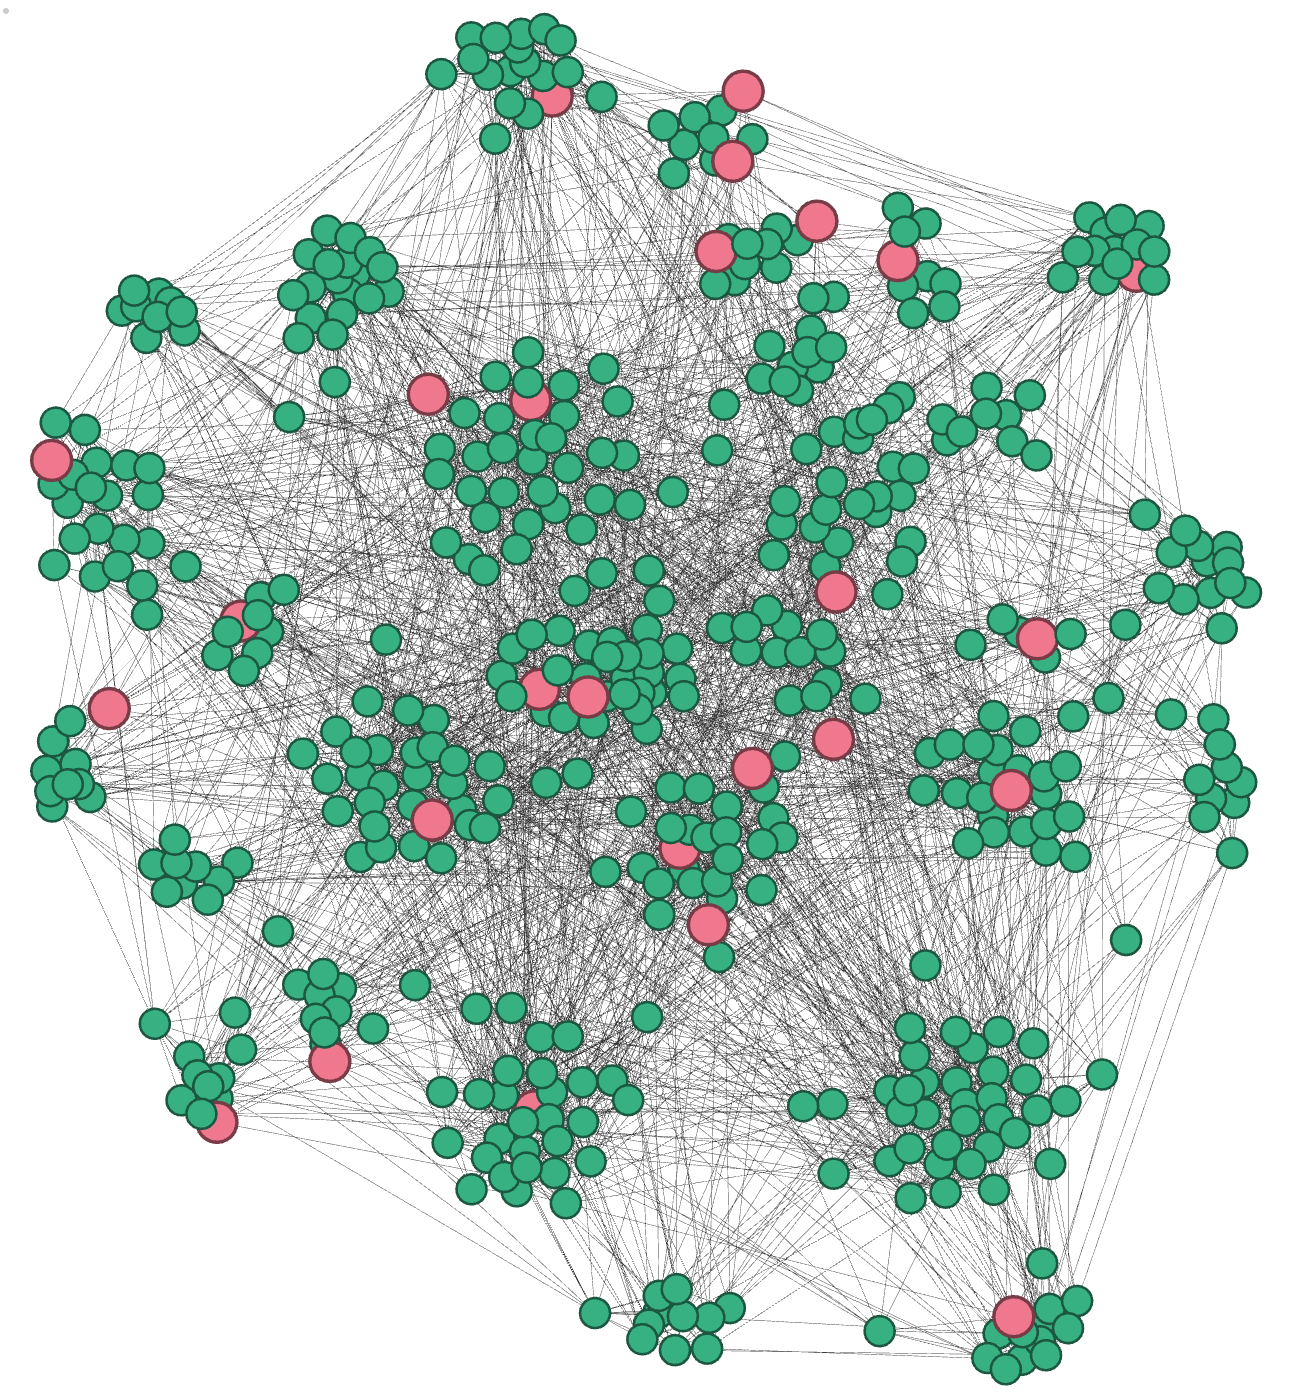
\includegraphics[width=\linewidth]{figures/begin1992.png}
\end{minipage}%
\hfill%
\begin{minipage}{.3\linewidth}
    \centering
    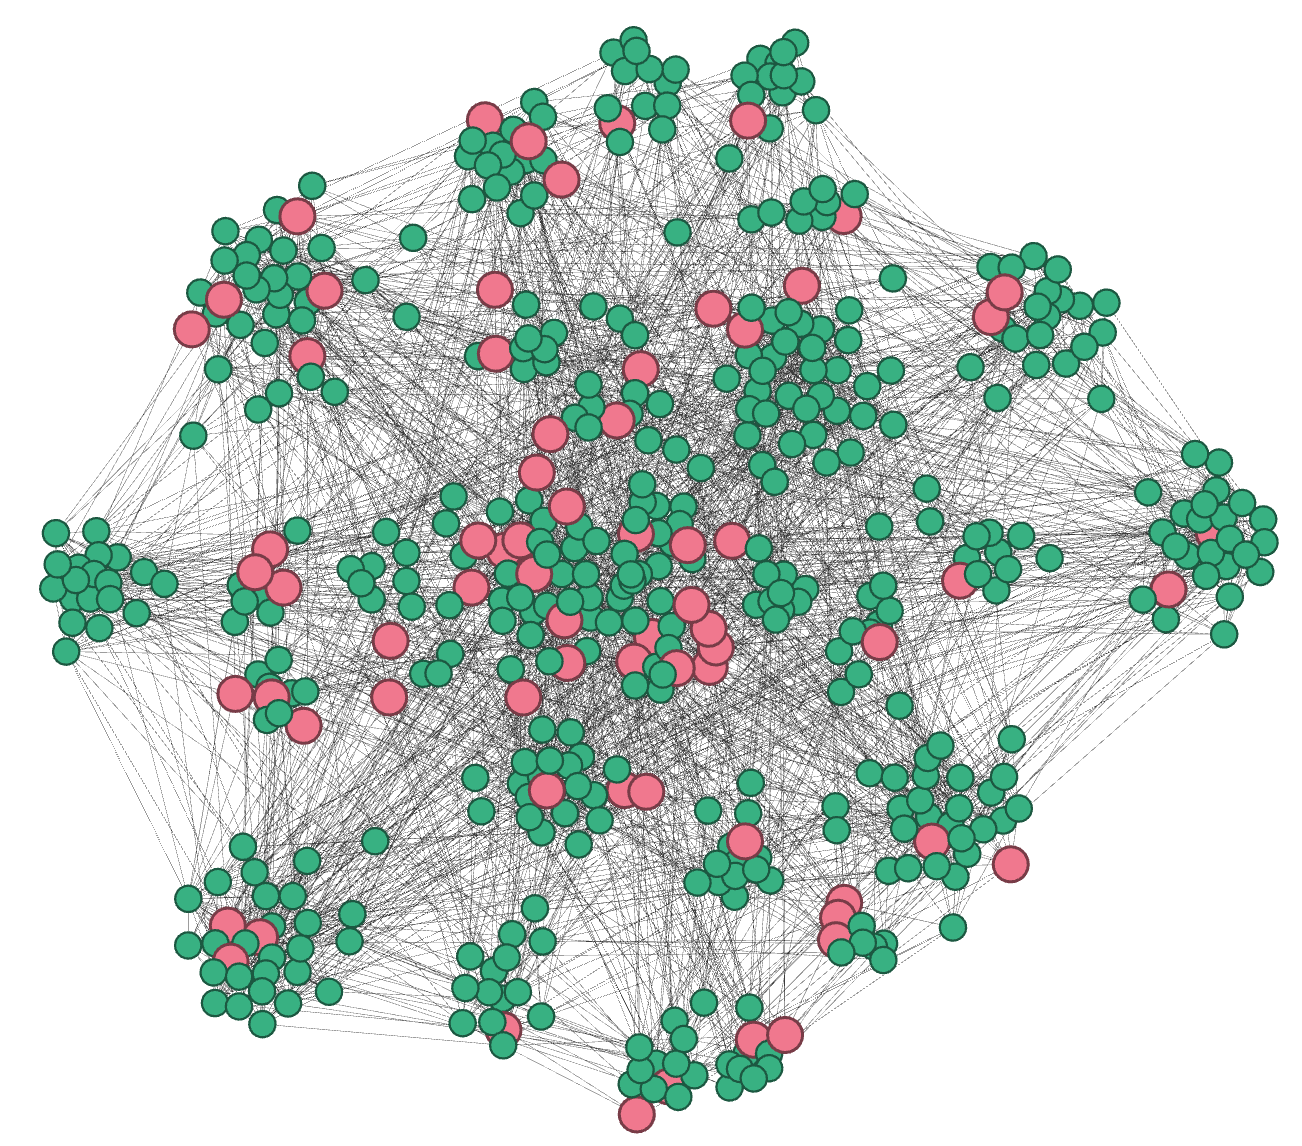
\includegraphics[width=\linewidth]{figures/end2017.png}
\end{minipage}%
\hfill%
\begin{minipage}{.3\linewidth}
    \centering
    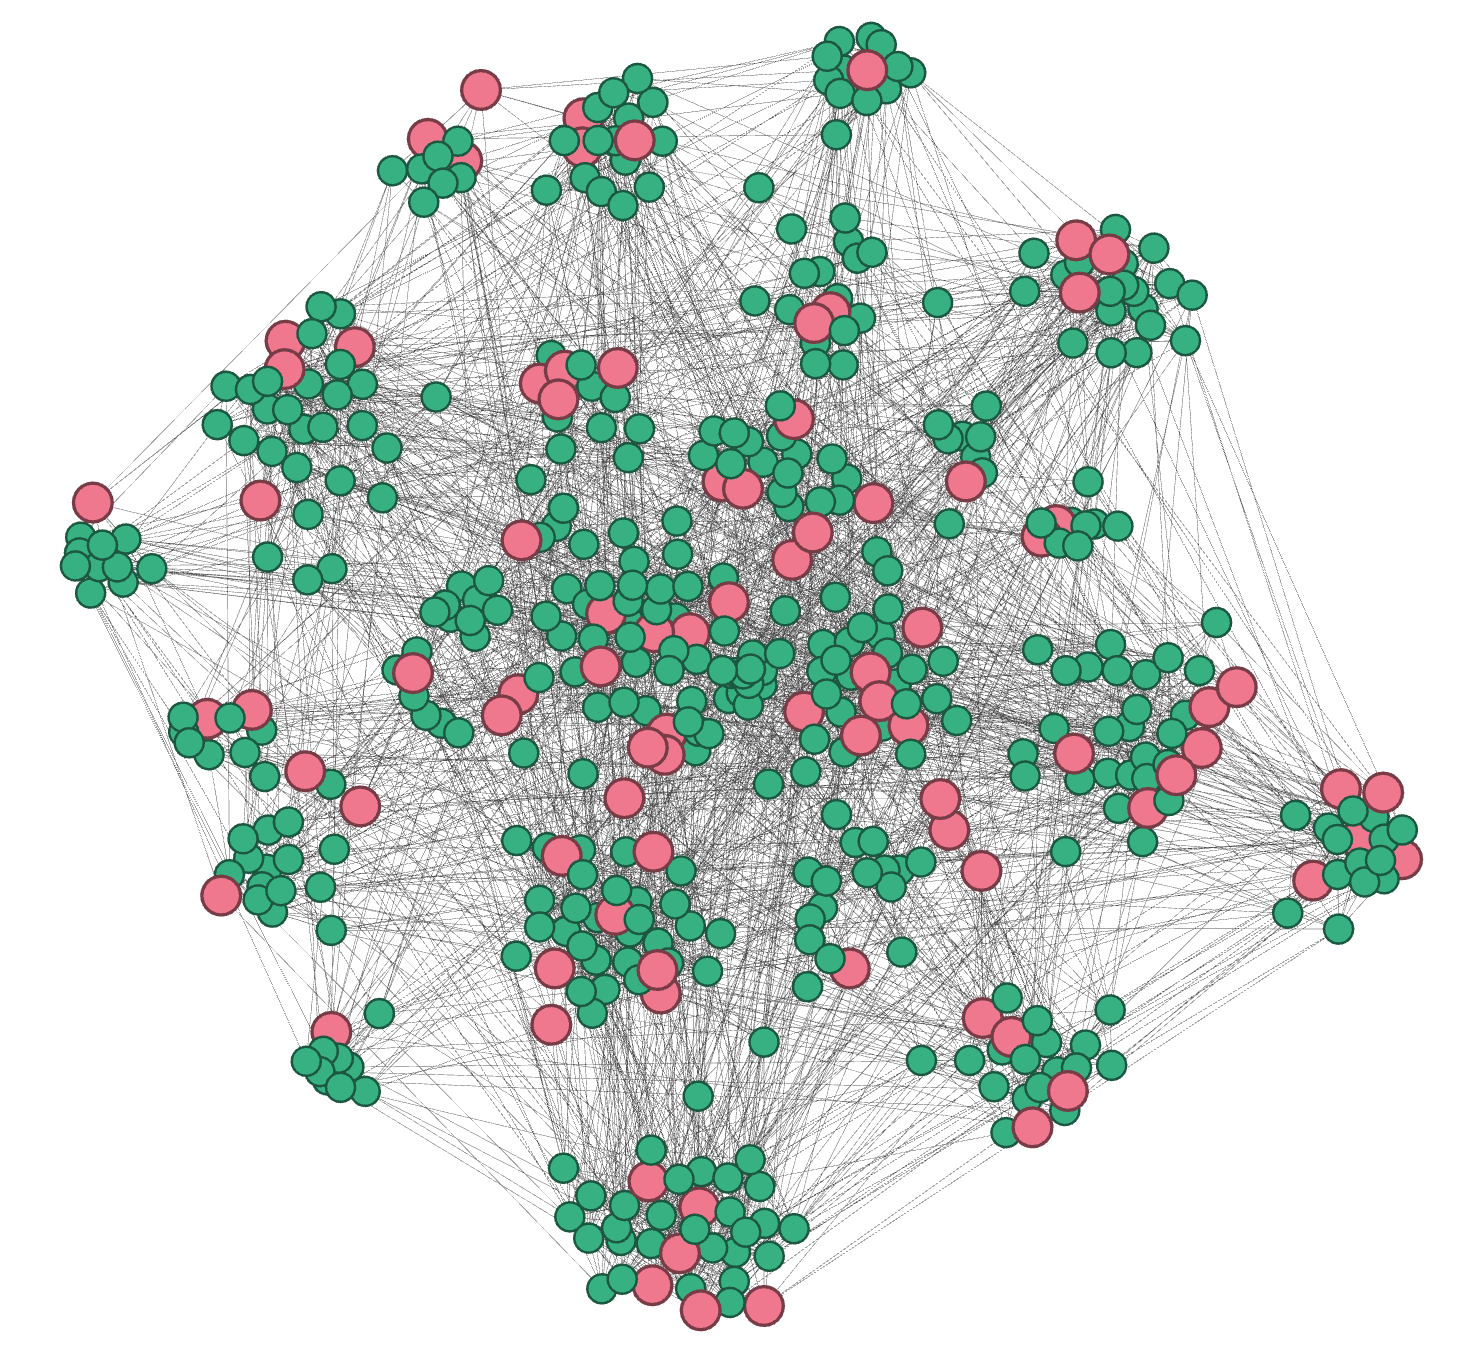
\includegraphics[width=\linewidth]{figures/end2042.png}
\end{minipage}%
\hfill%
\begin{minipage}[t]{.3\linewidth}
    \caption{\label{fig:begin1992} \textbf{Initial Network in 1992}. Nodes represent obese (red) or non-obese (green) agents which are connected by edges corresponding to their social connections. The rate of obesity is \(5.2\%\) \cite{bmistatistics}, and obese agents are randomly distributed.}
\end{minipage}%
\hfill%
\begin{minipage}[t]{.3\linewidth}
    \caption{\label{fig:end2017} \textbf{Reconstruction of the Swiss Evolution}. The network from Figure \ref{fig:begin1992} after 25 time-steps, with transmission rate $\beta = 0.005 $ and recovery rate $\gamma_0 = 0.023$ and spontaneous rate $\alpha_0 = 0.006$ obtained from non-linear least squares that best model the Swiss evolution of obesity. The rate of obesity is \(13.4\%\)).}
\end{minipage}%
\hfill%
\begin{minipage}[t]{.3\linewidth}
    \caption{\label{fig:end2042} \textbf{Prediction of the Obesity Rate inn 2042}. The network from Figure \ref{fig:end2017} after another 25 time-steps, with $\beta = 0.005 $, $\gamma_0 = 0.023$ and $\alpha_0 = 0.006$. The rate of obesity is \(17.4\%\)).}
\end{minipage}%
\end{figure}

\FloatBarrier

\subsection{Parameter Dependence and Reconstruction of the Evolution of Obesity in Switzerland}

We generate a network of 500 agents using the obesity rates of the Swiss population in 1992 \cite{bmistatistics} as described in section \ref{section:generating-network}. Red (green) nodes represent obese (non-obese) agents. Therefore the ratio between red and green nodes corresponds to the obesity rate of the network year. Note that here the obese agents are initially randomly distributed.
The generated network is shown in Figure \ref{fig:begin1992}. The age distribution and the gender of individual agents are not represented, as it is not relevant in our simplified model. Additionally, since only one type of social connection between agents is considered, there is no meaning behind the color of edges. \\

\begin{figure}[!htb]
    \centering
    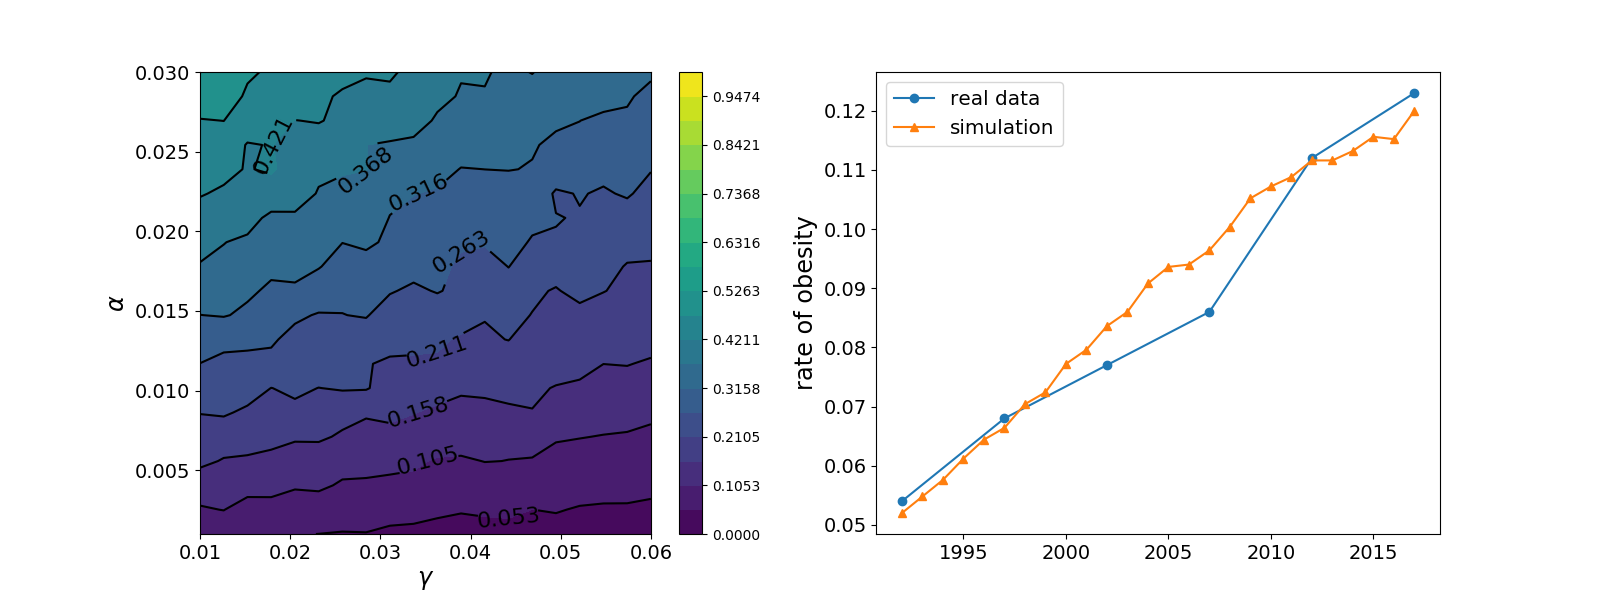
\includegraphics[width=\linewidth]{figures/parameters-25y.png}
\begin{minipage}[t]{.45\linewidth}
    \caption{\label{fig:parameters-25y} Obesity rate after 25 time-steps as a function of recovery rate $\gamma$ and spontaneous rate $\alpha$. The initial obesity rate is 5.2 \% and the transmission rate $\beta=0.005$}
\end{minipage}%
\hfill%
\begin{minipage}[t]{.45\linewidth}
    \caption{\label{fig:comparison} Comparison between the evolution of the obesity rate during 25 years with the real data of the Swiss population between 1992 and 2017. The simulation is run with $\beta = 0.005 $, $\gamma_0 = 0.023$, $\alpha_0 = 0.006$ and an initial obesity rate of 5.2 \%}
\end{minipage}%
\end{figure}

\FloatBarrier
Parameter dependency analysis is performed to examine the impact of varying rates \(\gamma, \alpha\) on the final rate of obesity in simulations. We keep the transmission rate \(\beta\) constant at a value of \(0.005\) as found in \cite{infectiousDiseaseModeling}. While this rate was found to fit the population studied in the US, the corresponding rate in Switzerland would most likely be different. Nevertheless, this is a simplification made in our model, since we assume that Switzerland and the US do not differ in that regard as strongly as in the other two rates. We run simulations for pairs of varying rates \(\gamma, \alpha\) and plot them against the rates of obesity produced by simulations using those rates. The recovery and spontaneous infection rates used for this analysis are twenty linearly spaced values between \(0.01\) to \(0.06\), and between \(0.01\) to \(0.03\) respectively. For each pair of parameters, five simulations of 25 time steps are ran to model the development from 1992 to 2017. The average obesity rates in each time step of these five simulation are recorded. Figure \ref{fig:parameters-25y} shows the parameter dependence between \(\gamma, \alpha\) and the average final rate of obesity in the network. \\

A non-linear least squares approach is then used to find the pair of parameters that best fits the development of obesity in Switzerland\cite{bmistatistics}. Consider for this a fixed pair of parameters \((\gamma_i, \alpha_j)\). The residual for every year \(1992, 1997, 2002, 2007, 2012,\) and \(2017\) is then defined as the difference between the actual rate of obesity in Switzerland in the given year and the average rate recorded in the corresponding time step of the simulations using \(\gamma_i, \alpha_j\) recorded previously. These residuals are then squared and summed over all six years. Finally, we choose the pair of parameters with the lowest square sum of residuals, which is then the least squares solution that best fits our data. \\

Using this approach, we obtain the values \((\gamma_0 = 0.023, \alpha_0 = 0.006)\) as the solution, with a sum of squared residuals $\epsilon = 1.63 \cdot 10^{-3}$. Figure \ref{fig:comparison} shows the evolution of the obesity rate in Switzerland along with the simulated evolution obtained using \(\gamma_0\) and \(\alpha_0\). Indeed, we observe similar trends. \\

The final network obtained by simulations using $\gamma_0$ and $\alpha_0$ is shown in Figure \ref{fig:end2017}, with an average obesity rate of 13.4\%. Here, one can observe the formation of clusters with prevalence of either obese or non-obese agents as described in \cite{spreadOfObesityPaper}.

\subsection{Predicting the Future Rates of Obesity in Switzerland}

Supposing that recovery and spontaneous rates remain constant over the next 25 years, we use our model to make predictions about the future evolution of obesity in Switzerland. Figure \ref{fig:end2042} shows the final network obtained in section 5.1 after another 25 time steps using the network from Figure \ref{fig:end2017}. The final obesity rate our model produces on average is 17.4\%.

\newpage

\section{Conclusion and Outlook}

Despite the simplifications our model was subjected to, and the limited set of parameters we utilised, we find that we extract spontaneous and recovery rates that in terms of order of magnitude, are highly in line with those found in research papers pertaining population studies in the US \cite{infectiousDiseaseModeling}. While in our simulations we arrive at a spontaneous rate of 0.006 and a recovery rate of 0.023 (with fixed transmission rate of 0.005), the research conducted in \cite{infectiousDiseaseModeling} result in a spontaneous rate of 0.02 and a recovery rate of 0.04. For what it's worth, our lower rates seem logical considering the general obesity prevalence in Switzerland is lower than that of the USA. The  fact that our rates seem appropriate and reasonably in line with those of other independent research results, hints at the possibility that the theory of a social contagion holds water, indeed. \\

Furthermore, bearing in mind the number of simplifications we made, we find there are numerous ways our model can be expanded upon: one may begin to differentiate between different kinds of relationship (friendship, family, etc.)\cite{spreadOfObesityPaper} or utilise the fact that transmission rates can vary with the sex of a social contagion. Another caveat we had to work under was that our initial distribution of obese agents was completely at random: realistically, clusters should already have formed from the get-go in our baseline network. If we were to include all those considerations and worked these features into our simulations, we may inch even closer to the real rates and achieve an accurate prediction for 25 years down the line, provided this hypothesis of the existence of a social contagion is in fact proven true.\\

Should this indeed be the case, this would have wide-ranging consequences for society as we know it. We would find ourselves in a downward spiral of infections whereby more and more of the population will become obese and infect the social circles surrounding them which only exacerbates the issue even further. In our simplified model, we already predict obesity to rise as high as 17\% in 2042 with no break in this upward trend in sight. The conclusions needed to be drawn from this are that what we call an person's spontaneous/recovery rate must be lowered/increased, respectively, if we ever hope to curb this epidemic. Thus, the implications for society are that obese people must receive increased support in order to facilitate recovery and healthy individuals need to be more discouraged from contracting obesity "spontaneously", i.e. via improved education on the subject and promotion of more healthy lifestyles. 

\newpage

\section{Bibliography}

\bibliographystyle{plain}
\bibliography{refs}

\end{document}
